\section{Synthetic Detectors and the Grid}
\label{app:grid}
\begin{figure}[t]
\centering
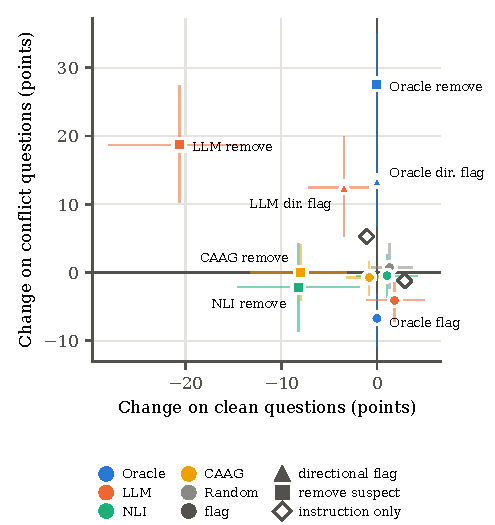
\includegraphics[width=\columnwidth]{generated/fig_tradeoff.pdf}
\caption{Change in one-way strict accuracy on RAMDocs conflict questions (y) against clean questions (x), relative to
no flags (gpt-4o-mini, default skeleton, confirmatory split, 95\% CIs). Colour: detector; shape: format. The oracle
sits on the y-axis because it never flags a clean question. Without direction, removal deletes the second passage of
each pair.}
\label{fig:tradeoff}
\end{figure}

\begin{figure*}[t]
\centering
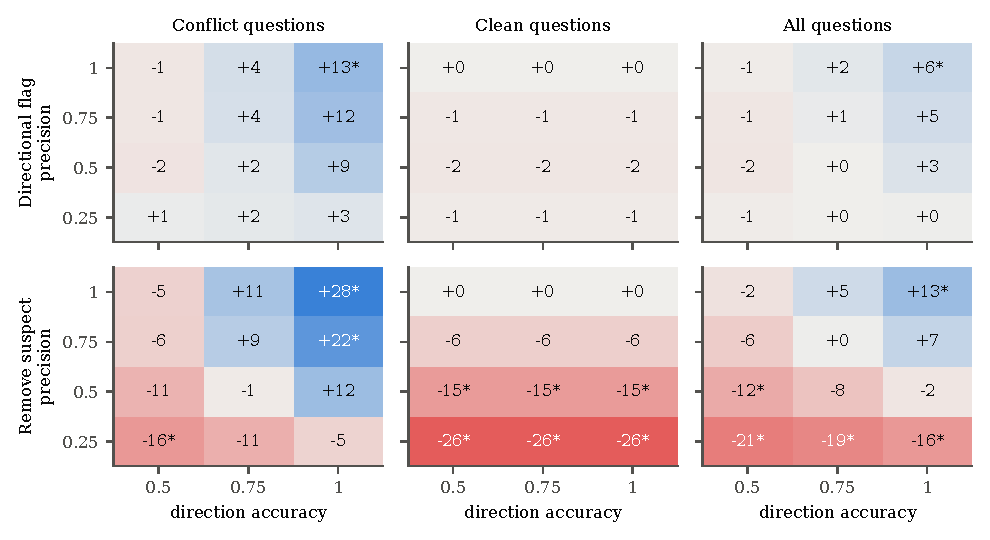
\includegraphics[width=\textwidth]{generated/fig_grid.pdf}
\caption{Synthetic detectors at recall 1: change in one-way strict accuracy (points) against no flags, by pair
precision (rows) and direction accuracy (columns), for the directional flag (top) and removal (bottom). $^*$:
significant after Holm correction over the 36 cells of that format and subset. Clean questions only see false flags,
so their rows do not vary with direction accuracy.}
\label{fig:grid}
\end{figure*}

\paragraph{Construction.}
We build each synthetic detector (Section~\ref{sec:synthetic}) from the gold labels. Each gold contradiction pair is
flagged with probability $r$. False flags are drawn from non-contradicting pairs at a single per-pair rate, set over
the whole split so that expected precision is $p$. Because the rate is dataset-wide, clean questions
receive false flags too. A true flag names the gold misinformation side with probability $d$, and otherwise the other side.
A false flag has no misinformation side, so its suspect is picked uniformly. Each pair gets one uniform draw for
flagging and one for direction, and every cell reuses them. Cells are therefore nested: raising $r$ or $d$, or
lowering $p$, only adds flags or corrections. The nesting keeps comparisons across cells paired.

\paragraph{Gains rise with direction accuracy; precision matters mainly for removal.}
Figure~\ref{fig:grid} replaces the oracle with synthetic detectors of known quality. Gains rise with direction
accuracy in both formats. Only the cells with perfect direction are significant on all questions (directional flag
\gDirOneDOneAll, removal \gRemOneDOneAll\ points at perfect precision). Neighbouring cells at direction accuracy
0.75 have similar point estimates on conflict questions, so the pattern is a dose-response, not a threshold. With 36 cells
under Holm, the grid has little power to separate adjacent levels.

Precision matters mainly for removal. On clean questions a cell's prompt does not depend
on direction accuracy, so the false-flag cells reduce to \hFourRemN\ distinct comparisons per format. Removal is
significantly harmful in \hFourRemHarm\ of them, the directional flag in \hFourDirHarm\ (H4a). Under removal, false flags
delete correct passages, which costs clean questions \agRemHalfDOneClean\ points at precision 0.5 and
\agRemQuDOneClean\ at 0.25, while synthetic false directional flags cost at most two points. The harm tracks the
share of clean questions that lose a correct document (Spearman $\rho=\hFourRho$ over \hFourRhoCells\ distinct
cells, 95\% CI \hFourRhoCI\ from a question-level bootstrap; H4b). Removal hurts clean questions significantly more
than the directional flag in \hFourRemWorse\ of \hFourMatched\ matched cells (H4c; we set no threshold, so we report
the count). Removal is the more powerful and the more fragile format: its best cell gains twice the directional
flag's on all questions, but below precision 0.75 it is the only format that does net harm.


\paragraph{Placing real detectors on the grid.}
\label{sec:placement}
Can the grid predict a real detector's effect from a few summary numbers? We compare two ways of summarising a
detector. \emph{Pair-level}: its pair precision, recall and direction accuracy. \emph{Document-level}: what it does
to each subset's documents in a given format. For conflict questions, that is the share whose misinformation documents
are all marked and the share that have a correct document marked; for clean questions, the share that have a correct
document marked. Here ``marked'' means removed (remove) or headed as misinformation (directional flag). The prediction
for a subset is the inverse-distance-weighted mean effect of the four nearest grid cells in that space.

\paragraph{Both summaries place most real effects inside the prediction interval.}
If the grid only described synthetic detectors, it would be of limited use. Figure~\ref{fig:placement} (Appendix~\ref{app:extra}) tests
whether it predicts real ones (H6). As pre-registered, we bootstrap the whole prediction (cell effects, every detector's
location and the interpolation) over questions, and ask whether the actual effect falls inside the 95\% interval.
Document-level locations put \hSixDocIn\ of \hSixN\ effects inside, and pair-level locations
\hSixPairIn. Document-level errors are smaller on
average (\hSixDocMae\ vs.\ \hSixPairMae\ points), but the paired difference, \hSixMaeDiff\ \hSixMaeDiffCI\ (exact
sign-flip $p=\hSixMaeP$), is not significant over \hSixN\ cases. Both spaces miss the same case, the LLM detector's
removal gain on conflict questions: one correctly directed pair is enough to remove a misinformation document, so the
detector removes the misinformation on \misGoneLlm\% of conflict questions despite its low pair recall. We chose the
document-level axes after seeing the LLM detector on the pilot split. The grid is a useful first estimate of a
detector's effect, but with three detectors we cannot claim that one summary predicts better than the other.

